% Metabolomics

\lecture{A mixture model for metabolite peak identification}{Metabolomics}

\begin{frame}
	\frametitle{Metabolomics}
	\begin{itemize}
		\item Metabolome: the set of small molecule metabolites found within an organism.
		\begin{itemize}
			\item Hormones, sugars, etc 
		\end{itemize}
		\item Gives a reliable picture of the phenotype (\href{http://www.nature.com/ng/journal/v41/n2/abs/ng.308.html}{Fu et al 2009})
		\item But metabolites are hard to measure.
		\item Dominant paradigm is \ac{LC} \ac{MS}
	\end{itemize}
\end{frame}

\begin{frame}
	\frametitle{\ac{MS}}
	\centering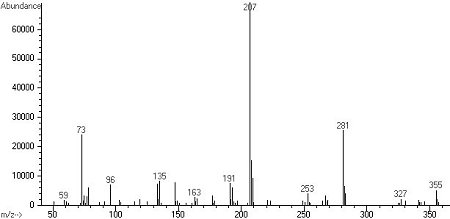
\includegraphics[width=0.5\linewidth]{spectra}
	\begin{itemize}
		\item Output of \ac{MS} is a set of mass-intensity pairs (peaks).
		\item Each peak corresponds to one ion.
		\item Each metabolite can result in many different ions:
		\begin{itemize}
			\item Different ions (i.e. $H^+,K^+$)
			\item Isotopes
		\end{itemize}
		\item All have predictable theoretical mass (for particular metabolite)
	\end{itemize}
\end{frame}

\begin{frame}
	\frametitle{\ac{LC}/\ac{MS}}
	\begin{multicols}{2}
		\begin{itemize}
			\item Most samples are too complex for a single \ac{MS} analysis
			\item First \emph{separate} the sample via \ac{LC}
			\item Perform many \ac{MS} analysis at different \ac{RT}
		\end{itemize}
		\newpage
		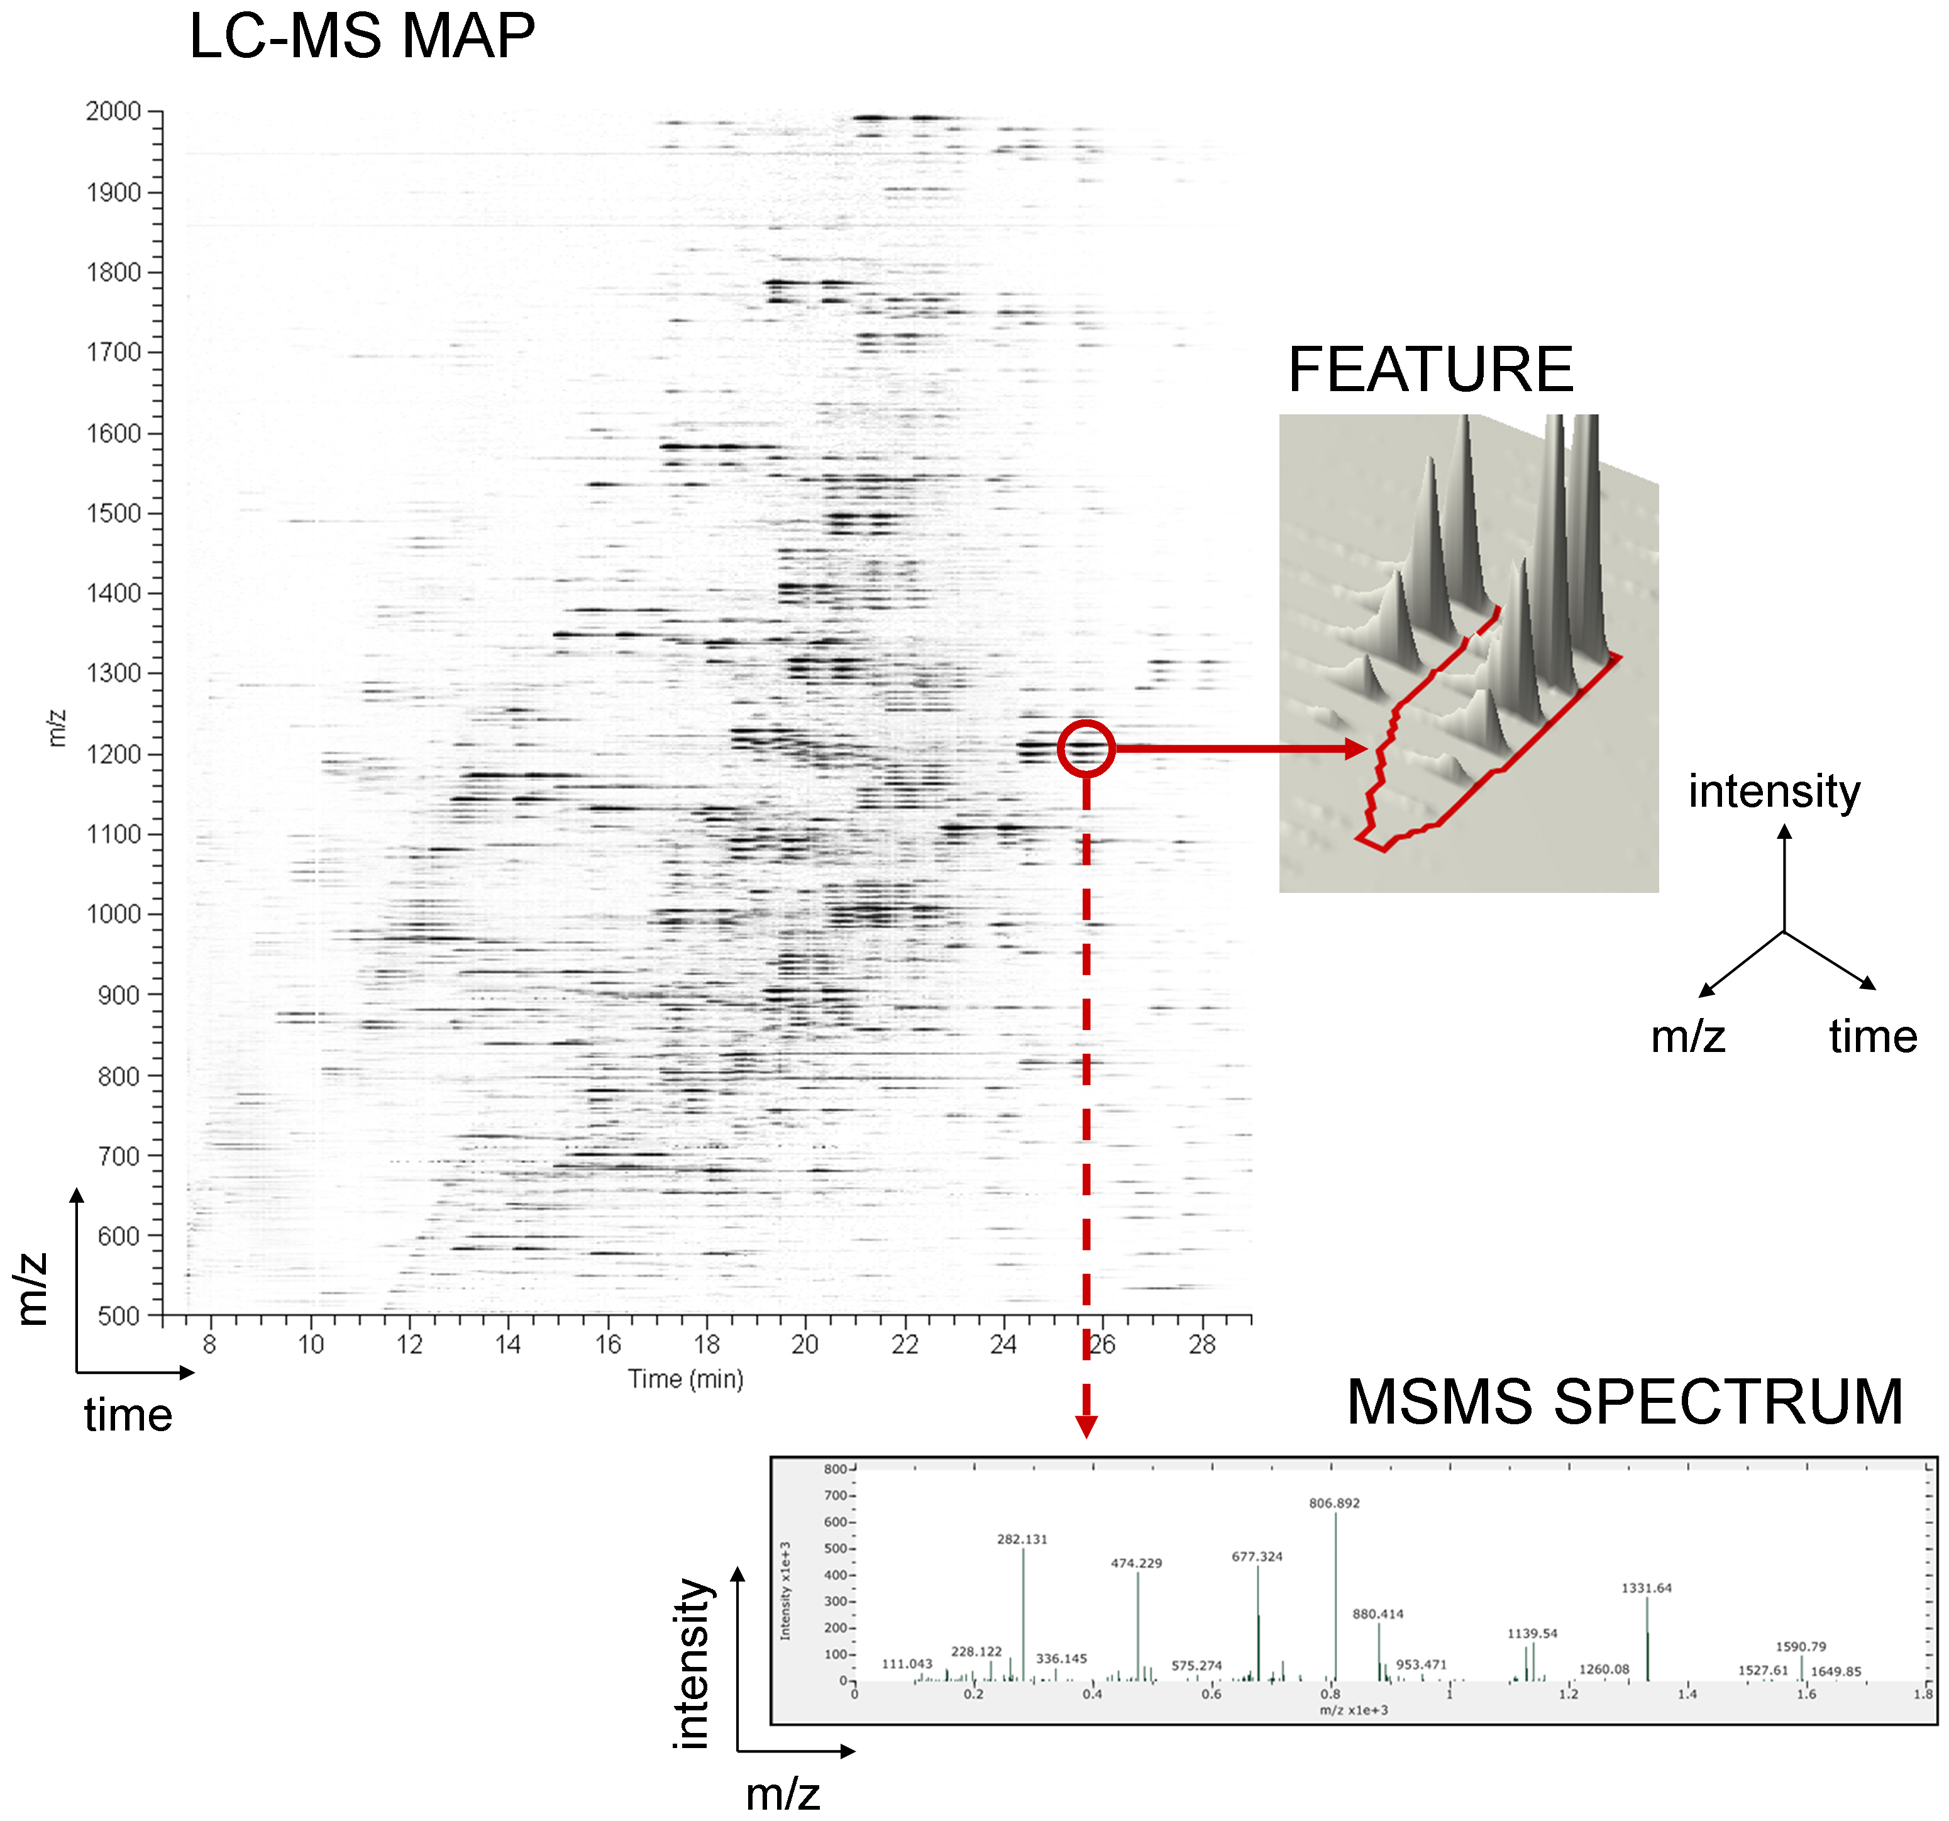
\includegraphics[width=\linewidth]{lcms}\\
		\href{http://www.beilstein-institut.de/glycobioinf2009/ProceedingsWeb/Peltoniemi/Peltoniemi.html}{(image from Peltoniemi et.~al)}
	\end{multicols}
\end{frame}

\begin{frame}
	\frametitle{What are the peaks?}
	\begin{itemize}
		\item How do we identify things in this 2D image?
		\item Doing each peak separately (traditional approach; searching mass against a database) leads to many false positives
		\item Can we use the fact the relationships between all peaks from the same metabolite to improve identification?
	\end{itemize}
\end{frame}

\begin{frame}
	\frametitle{Relationships between peaks}
		\begin{itemize}
			\item Retention time:
			\begin{itemize}
				\item All peaks derived from the same metabolite will elute at roughly the same time
			\end{itemize}
			\item<2-> Mass:
			\begin{itemize}
				\item For a particular chemical formula we can work out what all the adduct peaks (e.g. M+H) will be
				\item No known relationship between different adducts [might be worth investigating]
			\end{itemize}
			\item<3-> Intensity:
			\begin{itemize}
				\item The isotope peaks for a particular adduct have well defined relative intensities
			\end{itemize}
		\end{itemize}
\end{frame}

\begin{frame}
	\frametitle{MetAssign}
	\centering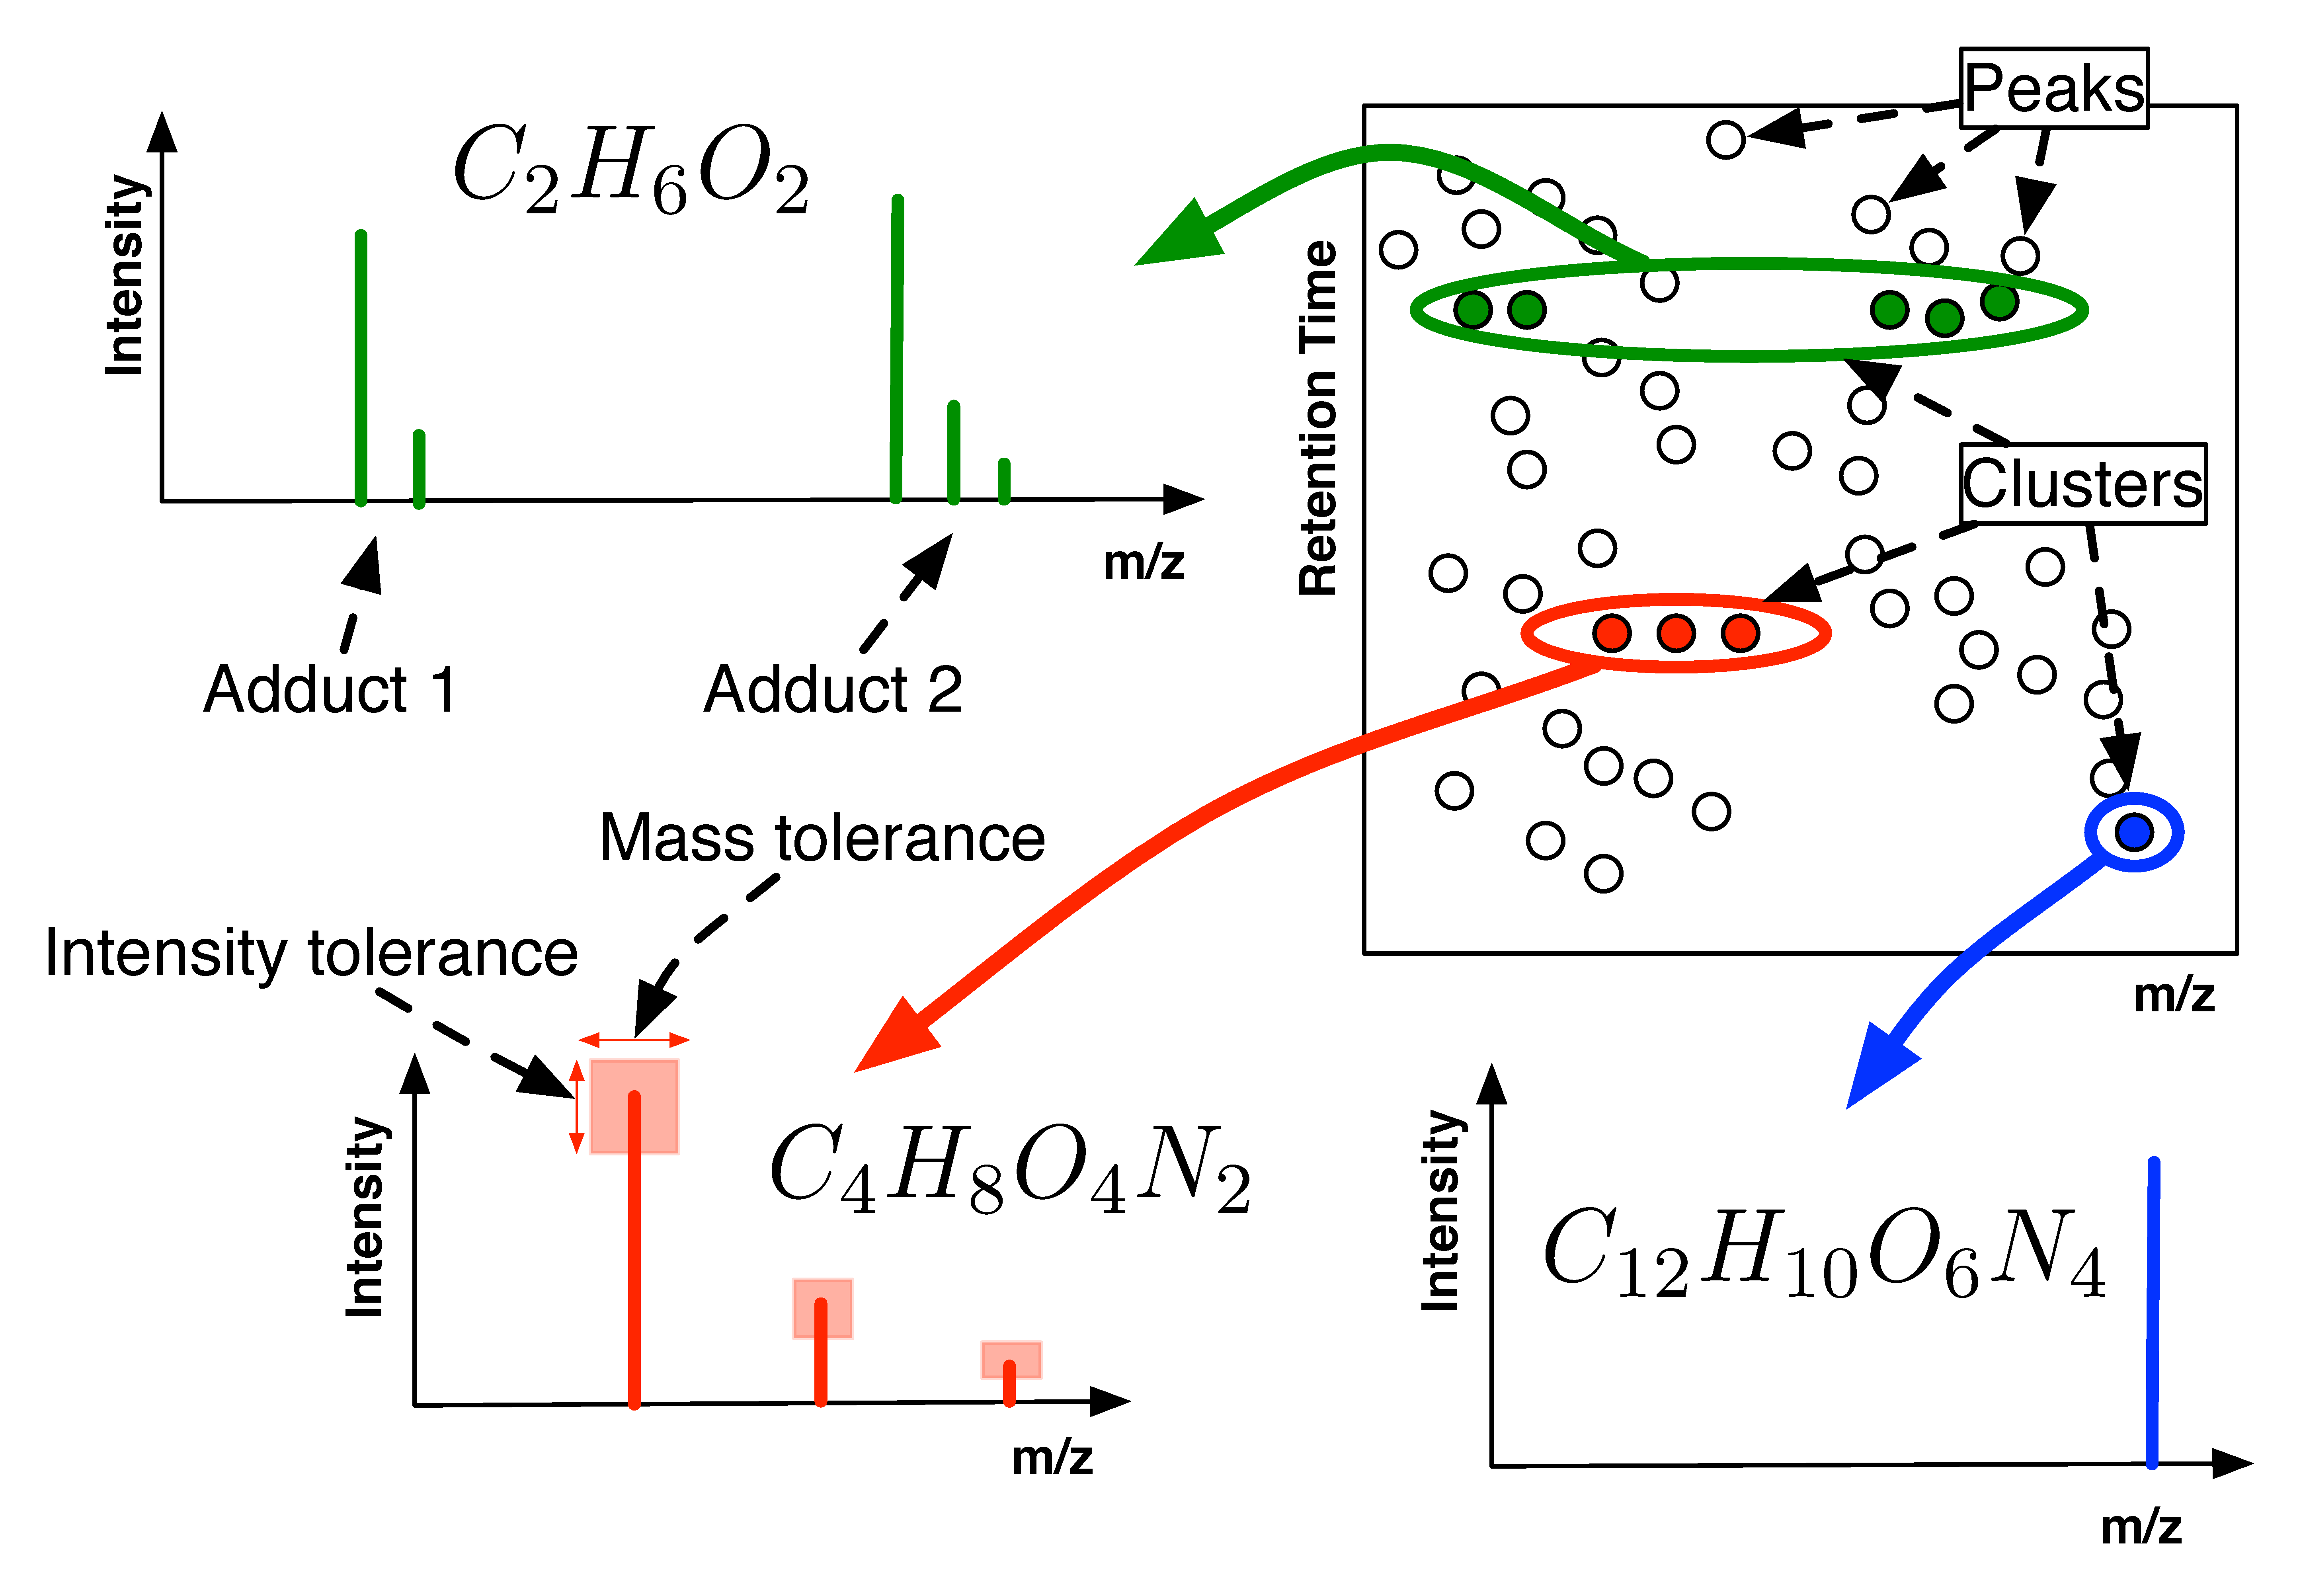
\includegraphics[width=\linewidth]{model-cartoon}
\end{frame}

\begin{frame}
	\frametitle{MetAssign}
	\begin{itemize}
		\item Use a DP mixture model
		\item Each cluster is linked to a particular chemical formula (from database)
		\item Likelihood has terms for:
		\begin{itemize}
			\item RT: all peaks in cluster must have similar RT
			\item Mass: Must be from one of the possible masses for this formula
			\item Intensity: peaks within a particular adduct must have correct intensity relationship
		\end{itemize}
	\end{itemize}
\end{frame}

\begin{frame}
	\frametitle{MetAssign}
	\begin{itemize}
		\item Gibbs sampling
		\item At each Gibbs step, each peak is assigned to a cluster and the cluster to a formula
		\item Average peak to formula assignments over all samples
		\item Averaging over posterior clusterings
		\item<2-> Filtering:
		\begin{itemize}
			\item Access to posterior samples allows us to filter out obviously bad assignments (more later)
		\end{itemize}
	\end{itemize}
\end{frame}

\begin{frame}
	\frametitle{MetAssign}
	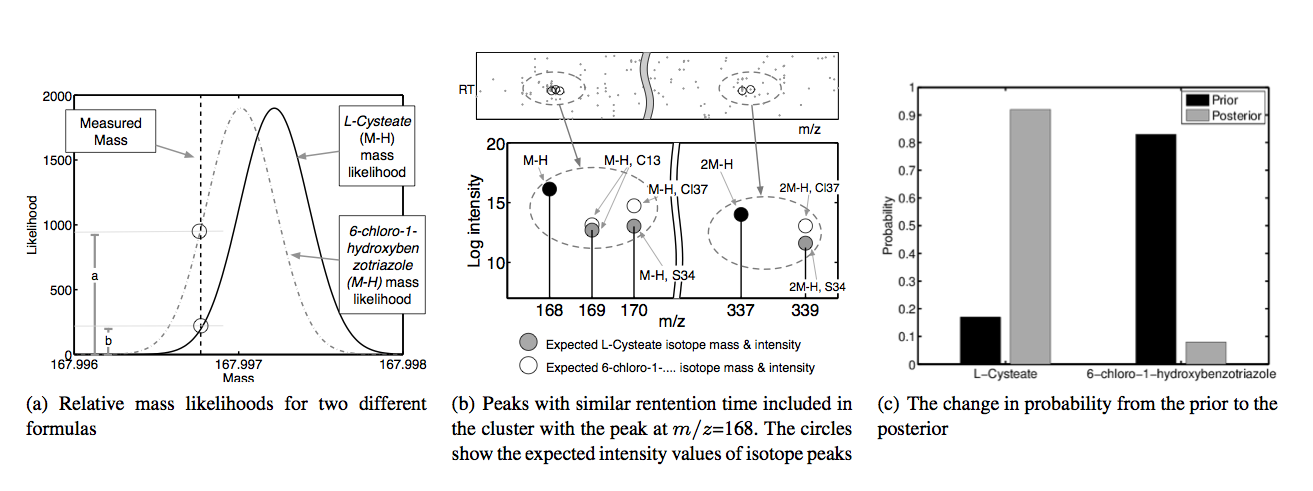
\includegraphics[width=\linewidth]{metassign}
	\begin{itemize}
		\item Database matches for each peak can be thought of as prior annotations
		\item After clustering we have posterior matches
		\begin{itemize}
			\item Note that by averaging over all clusterings we get posterior assignments for each peak.
			\item i.e. we are not interested in one clustering.
		\end{itemize}
	\end{itemize}
\end{frame}


\begin{frame}
	\frametitle{MetAssign}
	\centering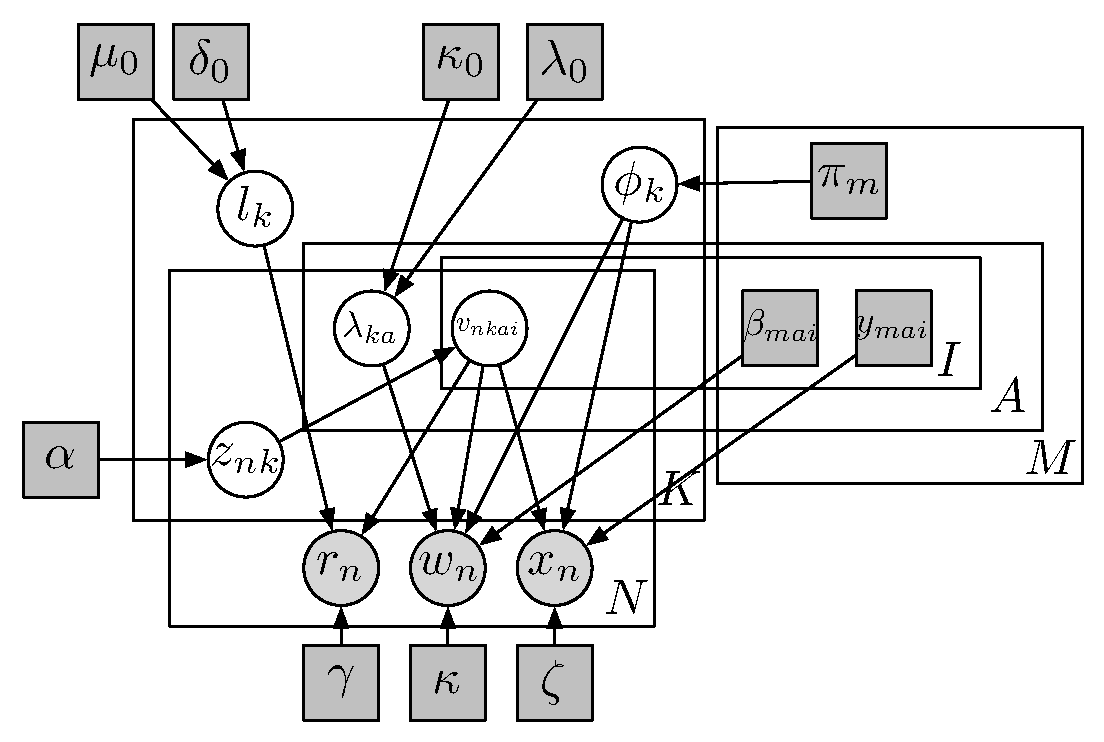
\includegraphics[width=\linewidth]{plates3}
\end{frame}

\begin{frame}
	\frametitle{MetAssign}
	\begin{itemize}
		\item Model consists of $K$ clusters
		\item Each cluster is linked to a metabolite from the database ($\phi_k$)
		\item The metabolite links lets us work out what masses ($y_{mai}$) and intensity relationships ($\beta_{mai}$) (for isotopes) we ought to see
		\item Each cluster has a retention time $l_k$
		\item Each adduct (ionisation type) has an intensity ($\lambda_{ka}$)
		\item $z_{nk}$ defines cluster membership for peak $n$
		\item $v_{nkai}$ defines membership within the cluster
	\end{itemize}
\end{frame}

\begin{frame}
	\frametitle{MetAssign: inference}
	\begin{itemize}
		\item Gibbs sampling updates are all fairly straightforward (assuming Gaussian noise everywhere)
		\item Can also include Metropolis-Hastings steps for changing which metabolite a cluster is assigned to
		\item Proportion of times a peak is assigned to a metabolite (via a cluster) gives posterior probability
		\item Access to posterior samples lets us do useful things
		\begin{itemize}
			\item e.g. only consider assignments of peaks if all bigger isotope peaks are present
		\end{itemize}
	\end{itemize}
\end{frame}

\begin{frame}
	\frametitle{MetAssign: results}
	\centering\includegraphics<1>[width=\linewidth]{metassign_pr}
	\centering\includegraphics<2>[width=\linewidth]{metassign_roc}
\end{frame}

\begin{frame}
	\frametitle{Conclusions}
	\begin{itemize}
		\item Excellent performance (better than state of the art)
		\item \ac{DP} prior allows us to not fix number of metabolites \emph{a-priori}
		\item Probabilities are obtained by averaging over the clusterings
		\item Probabilistic assignments are useful for the experimenters
		\item Gibbs sampling is easy to implement (although a pain to make efficient)
	\end{itemize}
\end{frame}

\begin{frame}
	\frametitle{Problematic isomers}
	\begin{itemize}
		\item Unfortunately, some metabolites share chemical formulas but differ in structure
		\item Identifying them is very hard
		\begin{itemize}
			\item If they have different RT, current model will put them into different clusters linked to the same formula
			\item Can possibly identify them if we include additional information
			\item Even slight changes in probabilities would be useful
		\end{itemize}
	\end{itemize}
\end{frame}

\begin{frame}
	\frametitle{Additional information 1 - predicted RT}
	\begin{itemize}
		\item RT prior is currently fixed across all metabolites
		\item Easy to extend to be metabolite specific
		\item RTs can (kind of) be predicted with multi-variate regression
		\begin{itemize}
			\item Use predicted RTs as prior means for metabolites
			\item Tune the prior variance depending on how good the RT prediction is
		\end{itemize}
	\end{itemize}
\end{frame}

\begin{frame}
	\frametitle{Additional information 2 - metabolic networks}
	\begin{itemize}
		\item Metabolites do not exist in isolation
		\begin{itemize}
			\item They are the products of reactions involving other metabolites
		\end{itemize}
		\item<2-> This structure is useful for identification
		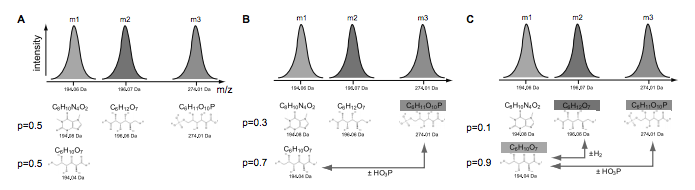
\includegraphics[width=\linewidth]{links}\\
		\href{http://dx.doi.org/10.1093/bioinformatics/btn642}{(Rogers et.~al 2009)}
		\item<3->Can incorporate this as a prior over metabolites to make more connected metabolites mode likely
	\end{itemize}
\end{frame}

\begin{frame}
	\frametitle{Future work}
	\begin{itemize}
		\item Incorporate predicted \ac{RT}
		% \begin{itemize}
		% 	\item It is possible to predict (badly) the \ac{RT} of a particular metabolite
		% 	\item Can easily be incorporated into the model through a metabolite-specific \ac{RT} prior
		% \end{itemize}
		\item<2-> Incorporate connectivity
		% \begin{itemize}
		% 	\item Metabolites live in networks (e.g. reactions)
		% 	\item We've previously used this to aid identification \href{http://dx.doi.org/10.1093/bioinformatics/btn642}{(Rogers et.~al 2009)}
		% 	\item Can be incorporated into the Metropolis-Hastings step to \emph{a-priori} make highly connected metabolites more likely
		% \end{itemize}
		\item<3-> Note: MetAssign currently under revision. When (if) published, search for `Rogers Daly Breitling metassign bioinformatics'
	\end{itemize}
\end{frame}		